\documentclass{article}

\usepackage{epsfig} \usepackage[margin=1.5in]{geometry}
\usepackage[semicolon,authoryear]{natbib} \bibliographystyle{natbib}
\usepackage{amsmath}
\usepackage{amsfonts}
\usepackage{cleveref}
\usepackage{verbatim}
\usepackage{graphicx}

\newcommand{\bO}{\mathcal{O}}
\newcommand{\argmin}[1]{\underset{#1}{\operatorname{arg\;min}}\;}

\title{Computational Methods for Principle Component Analysis Applied to
  Genotype Data}
\date{}

\begin{document}

\maketitle

\section{Introduction}

Ancestral history can be a influential confounder for the association between
genotypes and phenotypes (\cite{price}).
Thus stratification is needed to eliminate this bias.
Principle component analysis (PCA) has been proven to be useful in estimating
ancestral history (\cite{reich}).
The standard way of doing PCA is to find the principle components (PC) of the
reference data and project the data points of the study data onto them.
We call this method simple projection.
However, when the number of features are greatly larger than the size of the
reference sample,
the estimated PC scores by this method are known to be biased and less
than the populational PC scores.
One way of solving this issue is presented by \cite{wang}.
Their solution is to combine one study individual with the reference set and
find the PC scores of this augmented data set by singular value decomposition (SVD).
The study individual's PC scores is then retrieved from the PC score matrix and
mapped to the reference PC's by a Procrustes transformation.
We call this method ``augment, decompose, and transform (ADT).
This method has been shown to be useful in eliminating the shrinking bias of
study PC scores, but its disadvantage is computational inefficiency.

Two methods have been developed to solve this dillema of accuracy verses efficiency.
The magnitude and angle of shrinkage in simple projection has been calculated by
\cite{dey} and the result is implemented into the High Dimensional Principle
Component Analysis (HDPCA) package in R.
We call this method ``adjusted projection'' (AP).
The computational complexity of AP is significantly lower than that of ADT.
Moreover, an online SVD algorithm has been developed to speed up SVD by calculating an approximation of the top few PC scores only.
This is useful for our purpose since in genetic studies usually only the first few PC scores are needed. 
We call this method ``online augment-decompose-transform'' (OADT). 

In addition, we aim at solving a problem with finding the PC's of the reference set.
The previously mentioned four methods all need to find the SVD of the reference data first.
This requires loading the covariance matrix of the reference data into the
computer's memory. 
However, when the size of the reference set is large,
the resulted covariance matrix will far exceed the size of a normal personal
computer's memory.
To solve this issue, a randomized SVD method has been developed that does not
require finding the covariance matrix.

In this paper, we compare the theoretical and empirical properties of simple
projection, augment-decompose-transform, adjusted projection, and online augment-decompose-transform. In particular, we are
interested in their computational complexity as well as empirical speed and
accuracy.
Secondly, we compare using standard SVD and randomized SVD for the reference set
and examine the difference in accuracy and runtimes.
We found that HDPCA projection and OADT have both achieved the accuracy of ADT
and the efficiency of simple projection.
In addition, randomized SVD gives results similar to standard SVD and only
increase the computational time for the reference data.





\section{Method}

\subsection{Model}

\subsubsection{Data Format}
As mentioned previously, there are two datasets: a reference set and a study
set.
They are both represented as matrices.
A data matrix contains the genotypes for the individuals.
Each row represents a single-nucleotide polymorphism (SNP),
while each column represents an individual.
Each entry of the matrix is $0$, $1$, or $2$,
representing the number of mutations observed at the SNP.
In our study, we only use the SNPs that are observed in both the reference and
the study group and have the same alleles.
Thus we have the same number of SNPs for both groups.
The genotypes of the reference group are stored in the $p \times n$ matrix $X$,
and those of the study group are stored in the $p \times m$ matrix $Y$.
For genotype data, it is common for $p$ to be significantly larger than $n$.
Thus we assume this to be true except for the part where we discuss the randomized SVD algorithm,
which is developed to handle datasets with exceedingly large $n$.

\subsubsection{Principle Component Analysis}\label{pca-intro}
  Given a multi-dimensional data, principle component analysis (PCA) looks for the directions in which the data has the greatest variance.
These unit vectors are called the principle components (PC's).
The PC's form an orthonormal basis for the sample space,
and we can ignore all but the first few PC's to reduce the dimension of the data.
In particular, let $X=UDV^T$ be the SVD of $X$,
where $U$ is a $p \times n$ matrix whose columns are the PC's,
$D$ is an $n \times n$ diagonal matrix storing the standard deviations of the PC's,
and $V$ an $n \times n$ matrix such that each row contains the standardized PC scores of an individual.
(Alternatively, we can use eigendecomposition to find the matrices since $X^T X = VD^2V^T$ and $X X^T = UD^2U^T$.)
We sort the diagonal elements of $D$ in descending order and rearrange the
columns of $U$ and $V$ accordingly.
We are interested in the top $k$ PC's (where $k \ll n$) and look at the top $k$
columns of $V$ for their PC scores.

\subsubsection{Estimating PC scores}

We assume that the reference data and the study data are generated from the same
population.
When the genotypes of all individuals of the population are given (which is very
unlikely in global genetic studies),
we use the method in \Cref{pca-intro} to find the PC scores of the individuals
we are interested in.
In practice, we have a reference dataset and a study dataset assumed to be generated from the
same population and use the former to estimate the populational PC scores of the latter.
There are several computational methods one can use to do this estimation.
In \Cref{sec:compu}, we compare the performance of four of them.

\subsection{Computational Methods}\label{sec:compu}



\subsubsection{Simple Projection (SP)}
The standard way for estimating PC scores is by projecting the study
individuals' data points to the PCs of the reference individuals.
We call this method ``simple projection'' (SP).
The algorithm goes as follows.

\begin{enumerate}
\item Compute $X^T X$.
  (Computational complexity: $\bO[n^2p]$.)  
\item Apply eigendecomposition to $X^T X$ to get $X^T X = V D^2 V^T$.
  ($\bO[n^3]$.)
\item Calculate $W = Y^T (X V D_1^{-1})$, where $Y$ is the data matrix for all the study individuals, $D_1$ the first $k_1$ columns of $D$. ($\bO[mpk_1 + pnk_1]$.)
\end{enumerate}

Total computational complexity: $\bO[n^2p + n^3 + mpk_1 + pnk_1)] \approx \bO[n^2p + mk_1p]$,
given that $k_1 \ll n \ll p$.

As the reference sample size increases,
the computational complexity of SP stays as a constant,
except for decomposing the reference matrix, which is done once for all study individuals.
However, it is known that the projection method tends to underestimates the magnitude of the PC scores when $n \ll p$,
which we call the ``shrinking bias''. (See \cite{dey}.)
This limits the accuracy of SP for high dimensional data.

\subsubsection{Augment, Decompose, and Transform (ADT)}

One way to solve the shrinking bias of SP is developed by \cite{wang}.
In this method, each study individual's data point is appended to the reference
data matrix.
Then SVD is applied to the augmented matrix,
and PC scores in this augmented sample are found for both the reference
individuals and the study individual.
The the PC scores of the reference individuals in this augmented sample is
compared with the PC scores of the reference individuals in the reference
sample,
which is calculated in the beginning,
and a linear (Procrustes) map is found to transform the latter into the former
with the smallest error.
This transformation is then applied to the PC scores of the study individual in
the augmented sample.
The resulted PC scores are used as an estimate for the study individual's
population PC scores.
Specifically, let
\[
  V =
  \begin{bmatrix}
    V_{\text{ref}} & W
  \end{bmatrix},
  \quad
  \tilde{V} =
  \begin{bmatrix}
    \tilde{V}_{\text{ref}} & \tilde{W}_\text{ref} \\
    \tilde{V}_\text{stu} & \tilde{W}_\text{stu}
  \end{bmatrix},
\]
where the dimensions of $V_\text{ref}$, $\tilde{V}_\text{ref}$, and $\tilde{V}_\text{stu}$ are $n \times k_1$, $n \times k_2$, and $1 \times k_2$, respectively, with $ 1 \leq k_1 \leq k_2 \leq n+1$. 
Next, we use Procrustes analysis to find
\[
  A, b = \argmin{A, b} d(V_\text{ref}, \tilde{V}_{\text{ref}}A+b)
\]
for some metric $d$.
Finally, we get the Procrustes-adjusted top $k_1$ PC scores for the study individual $V_\text{pro} = \tilde{V}_\text{stu} A + b$.
The algorithm is summarized as follows:
\begin{enumerate}
\item Compute $X^T X$.
  (Computational complexity: $\bO[n^2p]$.)  
\item Apply eigendecomposition to $X^T X$ to get $X^T X = V D^2 V^T$ (columns of $D$ and $V$ are sorted by PC variance with the first column corresponding to the greatest PC variance).
  ($\bO[n^3]$.)
\item Append $X^T y$ and its transpose to the last column and row of $X^T X$, respectively.
  The entry of the bottom-right corner is $y^T y$.
  This is exactly the same as computing $\tilde{X}^T \tilde{X}$,
  where $\tilde{X} = (X, y)$ is the reference group with the study individual added.
  ($\bO[np]$.)
\item Apply eigendecomposition to $\tilde{X}^T \tilde{X}$ to get $\tilde{X}^T \tilde{X} = \tilde{V} \tilde{D}^2 \tilde{V}^T$.
  ($\bO[n^3]$.)
\item Project the first $k_2$ columns of $\tilde{V}$ to the first $k_1$ columns of $V$ by using Procrustes analysis to get the transformed PC scores of the study individual (the last row of $V$),
  where $k_1 < k_2 \ll n$.
  (Computational complexity is ignorable if $k_2$ is not large compared to $n$.)
  \item Go to step 3 for the next study individual.
\end{enumerate}

Total Computational complexity: $\bO[n^2p + m(np + n^3)]$.

Although accurate, ADT is the slowest among the other three computational
methods.
Its computational complexity increases cubically as we increase the reference sample size to increase the accuracy of the PC scores.
The ADT method is has been implemented in the TRACE software by \cite{wang}.


\subsubsection{Adjusted Projection (AP)}

A more efficient way to solve the shrinking bias of SP is to estimate the
magnitude and angle of the shrinkage and adjust the study individuals' PC scores accordingly.
This method has been developed by \cite{dey} and implemented in the High
Dimension Principal Component Analysis (HDPCA) in the R language.
HDPCA reads the PC scores and variances calculated by projection and estimate the shrinkage factor to restore the unshrinked scores. 
The algorithm is
\begin{enumerate}
\item Compute $X^T X$.
  (Computational complexity: $\bO[n^2p]$.)  
\item Apply eigendecomposition to $X^T X$ to get $X^T X = V D^2 V^T$.
  ($\bO[n^3]$.)
\item Calculate $W = Y^T (X V D_1^{-1})$, where $Y$ is the data matrix for all the study individuals, $D_1$ the first $k_1$ columns of $D$. ($\bO[mpk_1 + pnk_1]$.)
  \item Input $D$ and $W$ to the pc\_adjust function in the HDPCA function to obtain the PC scores adjusted for the shrinking bias. ($\bO[p]$ for finding the number of distant spikes (function select.nspike), $\bO[n]$ for adjusting for the shrinking bias (function hdpc\_est))
\end{enumerate}

Total computational complexity: $\bO[n^2p + mk_1(p + n) + p + n] \approx \bO[n^2p + mk_1p]$,
given that $m$ or $n$ is large. The computational complexities between simple projection and adjusted projection are the same.
The accuracy of adjusted projection will be empirically shown later.

\subsubsection{Online ADT (OADT)}

A remedy for ADT is to reduce the computational complexity withou much sacrifice of the accuracy.
This is achieved by the online ADT (OADT) method.
Notice that in OADT, only the top $k_2$ PC's are used.
OADT uses the online SVD method, which calculates a close approximation of the first $k_3$ columns of $\tilde{V}$ for some $k_2 \leq k_3 \ll n$ and keeps everything else the same as in ADT, including Procrustes analysis. 
The algorithm is
\begin{enumerate}
\item Compute $X^T X$.
  (Computational complexity: $\bO[n^2p]$.)  
\item Apply eigendecomposition to $X^T X$ to get $X^T X = V D^2 V^T$.
  ($\bO[n^3]$.)
\item Calculate $U_3 = X V_3 D_3^{-1}$,
  where $V_3$ is the first $k_3$ columns of $V$,
  and $D_3$ is the diagonal matrix of the first $k_3$ diagonal entries of $D$.
  ($\bO[k_3 n p]$.)
\item Calculate 
  \[
    L = U_3^T y \quad \text{and} \quad K = y^T H,
  \]
  where $H$ is the normalized  $y - U_3L$
  ($\bO[k_3 p]$.)
\item Calculate $Q^T Q$, where
  \[
    Q = 
    \begin{bmatrix}
      D_3 & L \\
      0 & K
    \end{bmatrix}.
  \]
  ($\bO[k_3^3]$.)
\item Apply eigendecomosition to $Q^T Q$ to get $Q^T Q = \ddot{V}_3 \ddot{D}^2_3 \ddot{V}^T_3$.
  ($\bO[k_3^3]$.)
\item Calculate
  \[
    \tilde{V}_3 =
    \begin{bmatrix}
      V_3 & 0 \\
      0 & 1
    \end{bmatrix}
    \ddot{V}_3.
  \]
  ($\bO[nk_3^2]$.)
\item Project the first $k_2$ columns of $\tilde{V}_3$ to the first $k_1$ columns of $V$ by using Procrustes analysis to get the transformed PC scores of the study individual,
  where $k_1 < k_2  < k_3 \ll n$.
  (Computational complexity is ignorable if $k_2$ is not large compared to $n$.)
  \item Go to step 4 for the next study individual.
\end{enumerate}

Total computational complexity: $\bO[n^2p + n^3 + k_3np + m(k_3p + k_3^3 + nk_3^2]) \approx \bO[n^2p + m(k_3p + k_3^2n)]$, provided $k_3 \ll n \ll p$.

Here we see that the computational complexity of OADT for the study individuals increases linearly with respect to the reference sample size.
This makes the runtimes of OADT close to those of SP.
The closeness between the results given by OADT and ADT will be empirically shown later.

A comparison of computatinal complexities of the four PCA methods are shown in \Cref{tbl:cplx}.

\subsubsection{Randomized SVD}
In addition to estimating the PC scores of the study individuals,
we have another algorithm that aims at improving the decomposition of the
training data.
For SP, AP, ADT, and OADT, we need to find the covariance matrix of the training
data, which has dimension $n \times n$, and conduct eigendecomosition on it.
However, when $n$ is exceedingly large,
the covariance matrix cannot be loaded into the memory of an average personal
computer.
A randomized SVD (RSVD)algorithm has been developed to handle this issue.
RSVD is slower than standard SVD,
but it does not require loading the whole covariance matrix into the memory.



\subsection{Data}

In this study, we used both simulated data and real-life data to conduct
empirical tests of the computational methods for PCA.

\subsubsection{Simulation Studies}

We used the GGS software to simulate individuals migrating on a grid.
The parameters we chose to use are as follows:
\begin{enumerate}
\item L: Number of loci in each genealogy. (Fixed to $1000$.)
\item G: Number of genealogies. (Equal to $p / L$)
\item K: Side length of the grid. (Fixed to $2$.)
\item c: Number of haploids at each cell of the grid. (Equal to $2n / K^2$ and
$2m / K^2$)
\item M: Migration rate. (Fixed to $100$)
\end{enumerate}

For our study, we used different reference and study sample sizes.
First, we fix
the study size to be $m=200$ and increase $n$ from $1000$ to $3000$ with the
increment equal to $500$.
Next, we fix
the reference size to be $n=600$ and increase $m$ from $1000$ to $3000$ with the increment equal to $500$.

For comparing the speed of the algorithms,
we only compare the runtimes for the study individuals.
The time spent on calculations that are once-for-all (such as finding the SVD of
the reference matrix) is ignored.

For comparing the accuracy, we use two different measures.
First, for a given cell of the grid, we compute the mean of the PC scores of the 
reference individuals located at this cell.  
This is the estimated coordinate of the cell.
Next, we find the Euclidean distance between the estimated PC scores of the
study individuals and the estimated coordinates of the cells they are located
at.
These are the geographic estimation errors for the study individuals.
The average of these errors are used to measure the accuracy of the
computational methods (that is, the square root of the sum of squares divided by the
study size). 
Second, since ADT is believed to be the most reliable, we compare the average
Euclidean distance between the PC score estimates calculated by another method
to those calculated by ADT. 
This golden-standard error and the geographic error both range from zero to infinity.

The comparison of the runtimes and accuracy are conducted by using both the
standard SVD and randomized SVD on the training data matrix.

\subsubsection{Real-Life Datasets}

The real-life datasets used in our study are the UKBioBank and 1000 Genomes datasets.
They contain the genotype readings of individuals from different ethnic groups over the world.
For better comparison, we select only the SNPs that are included in both datasets,
the number of which is approximately $1.5 \times 10^5$.
We use the 1000 Genomes dataset as the reference and removed individuals who have at least one parent who is also in the dataset.
The reference samples size is approximately $2300$.
Moreover, we use the first 1000 individuals in the UKBioBank data set out of a
total number of $5 \times 10^5$ individuals. 
The measures we use for comparing speed and accuracy are the same as for
simulated data,
except that we do not use the geographic error here.
In addition, both the standard and randomized SVD on the training data set are tested.



\section{Results}

The predicted PC scores are shown in \Cref{fig:n1000} and \Cref{fig:ukb}.
For the comparison of the runtimes and accuracy for different reference and sample sizes for the simulated data,
see \Cref{fig:nChg} and \Cref{fig:mChg}.
For comparing the methods for the real-life data, see



\section{Discussion}

We find that AP improved the accuracy of SP without increasing the runtimes.
Moreover, OADT improves the speed of ADT without much sacrifice of accuracy.
In addition, randomized SVD is found to be as reliable as standard SVD in
calculating the PC's of the reference group.

\newpage

\begin{thebibliography}{}
 
\bibitem[Brand(2002)]{brand} Brand, M. (2002). Incremental singular value decomposition of uncertain data with missing values. {\it Computer Vision--ECCV 2002}, 707-720.

\bibitem[Dey \& Lee(2016)]{dey} Dey, R., \& Lee, S. (2016). Asymptotic properties of Principal Component Analysis and shrinkage-bias adjustment under the Generalized Spiked Population model. {\it arXiv preprint arXiv:1607.08647}.
  
\bibitem[Jolliffe(2002)]{jolliffe} Jolliffe, I. (2002). {\it Principal component analysis}. John Wiley \& Sons, Ltd.
Chicago	


 \bibitem[Wang et al.(2015)]{wang} Wang, C., Zhan, X., Liang, L., Abecasis, G. R., \& Lin, X. (2015). Improved ancestry estimation for both genotyping and sequencing data using projection procrustes analysis and genotype imputation. {\it The American Journal of Human Genetics, 96}(6), 926-937.

 \bibitem[Reich et al.(2008)]{reich} Reich, D., Price, A. L., \& Patterson, N.
   (2008). Principal component analysis of genetic data. {\it Nature genetics}, 40(5), 491.
   Reich, D., Price, A., Patterson, N (2008).
   Principle component analysis of genetic data. {\it Nature Genetics}

   \bibitem[Price et al.(2006)]{price} Price, A. L., Patterson, N. J., Plenge,
     R. M., Weinblatt, M. E., Shadick, N. A., \& Reich, D. (2006). Principal
     components analysis corrects for stratification in genome-wide association
     studies. {\it Nature genetics}, 38(8), 904.

\end{thebibliography}

\newpage

\begin{table} 
  \centering
  \begin{tabular}{|l|l|}
    \hline
    Method & Computational Complexity \\ 
    \hline
    Simple Projection (SP) & $\bO[n^2p + mk_1p]$ \\
    \hline
    Augment-Decompose-Transform (ADT) & $\bO[n^2 p + mn(p + n^2)]$ \\
    \hline
    Adjusted Projection (AP) & $\bO[n^2p + mk_1p]$ \\
    \hline
    Online Augment-Decompose-Transform (OADT) & $\bO[n^2 p + mk_3(p + k_3 n)]$ \\
    \hline
  \end{tabular}
  \caption{
    Comparison of computational complexity for the three methods.
    Here $p$ is the number of SNPs,
    $n$ is the number of individuals in the reference group,
    and $m$ is the number of individuals in the  study group.
    For projection, $k_1$ is the number of PCs needed
    For OADT, $k_3$ is the number of PCs calculated by online SVD, which is usually much less than $n$.}
  \label{tbl:cplx}
\end{table}

\begin{table} 
  \centering
  \begin{tabular}{|l|l|l|l|l|}
    \hline
    Method & Reference Runtimes & Study Runtimes & Reference Center Error & Golden Standard Error \\ 
    \hline
    Simple Projection (SP) &  \\
    \hline
    Augment-Decompose-Transform (ADT) & $\bO[n^2 p + mn(p + n^2)]$ \\
    \hline
    Adjusted Projection (AP) & $\bO[n^2p + mk_1p]$ \\
    \hline
    Online Augment-Decompose-Transform (OADT) & $\bO[n^2 p + mk_3(p + k_3 n)]$ \\
    \hline
  \end{tabular}
  \caption{
    Comparison of computational complexity for the three methods.
    Here $p$ is the number of SNPs,
    $n$ is the number of individuals in the reference group,
    and $m$ is the number of individuals in the  study group.
    For projection, $k_1$ is the number of PCs needed
    For OADT, $k_3$ is the number of PCs calculated by online SVD, which is usually much less than $n$.}
  \label{tbl:cplx}
\end{table}


\begin{figure}[p]
  \centering
  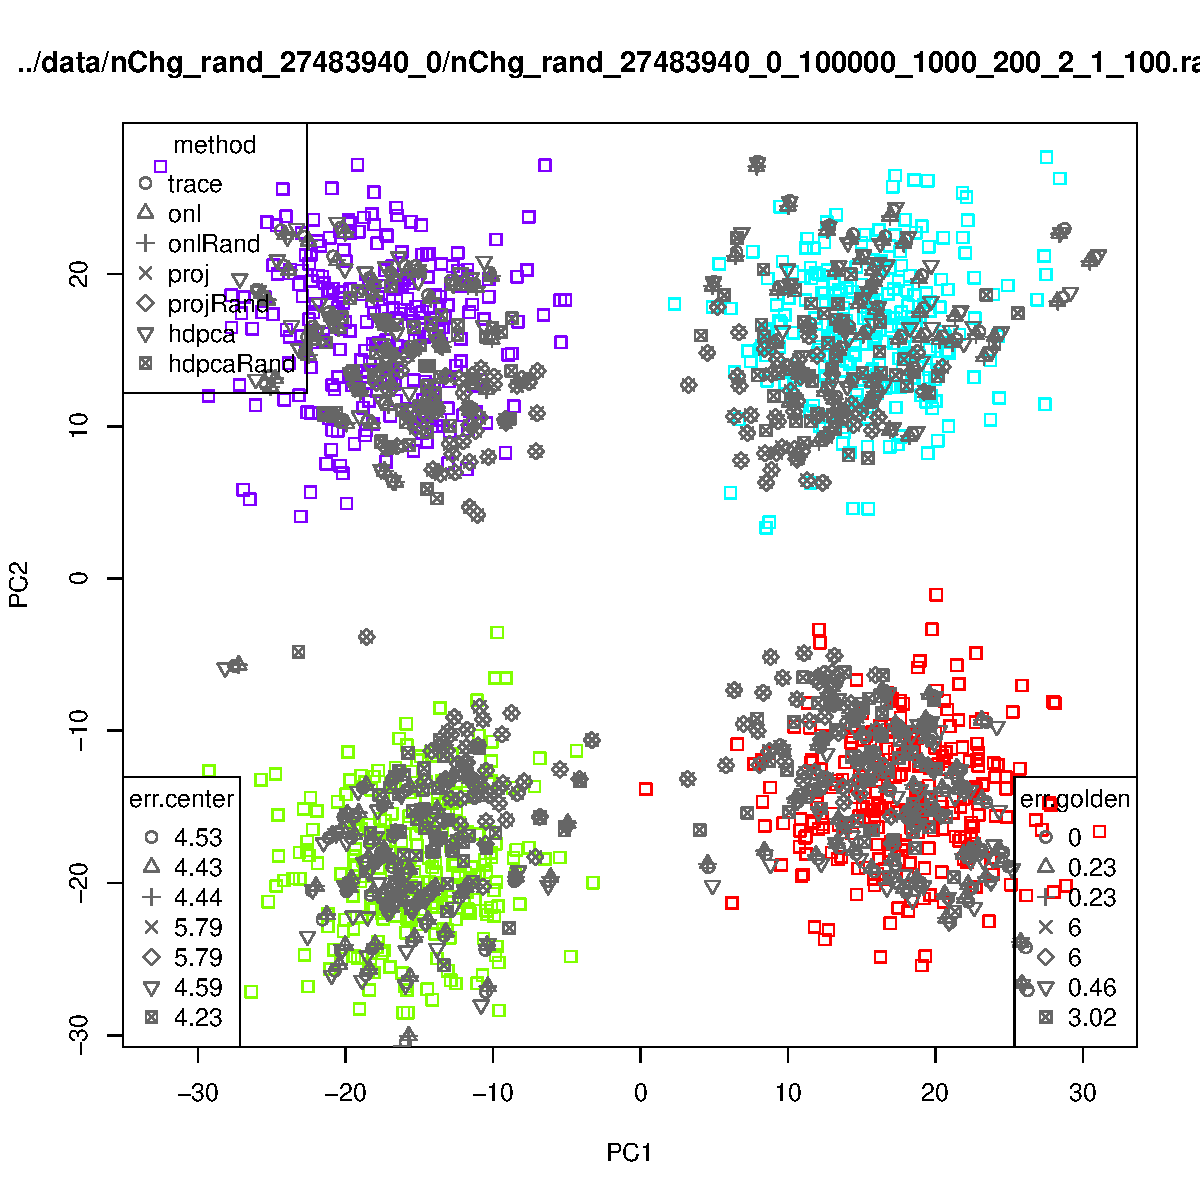
\includegraphics[width=0.98\textwidth]{n1000}
  \caption{
    Predicted PC scores on top of reference PC scores.
    The four populations in the $2 \times 2$ grid simulated by the GGS software can be clearly identified.
    Reference individuals are in color,
    while predicted PC scores for the study individuals are in gray.
    Two measurements of deviations (accuracy) are used.
    The reference center error is the square root of the average squared distance between the study individuals and the population centers, which are the means of the PC scores of the reference individuals by the populations.
    The golden standard error is the square root of the averate squared distance between the study individuals' PC scores predicted by different methods compared to the golden standard result, which in our case is the PC scores predicted by ADT.
    The reference size is 1000 and the study size is 200.
    There are 100,000 loci (1000 per genealogy) and the migration rate is 100.
  }
  \label{fig:n1000}
\end{figure}

\begin{figure}[p]
  \centering
  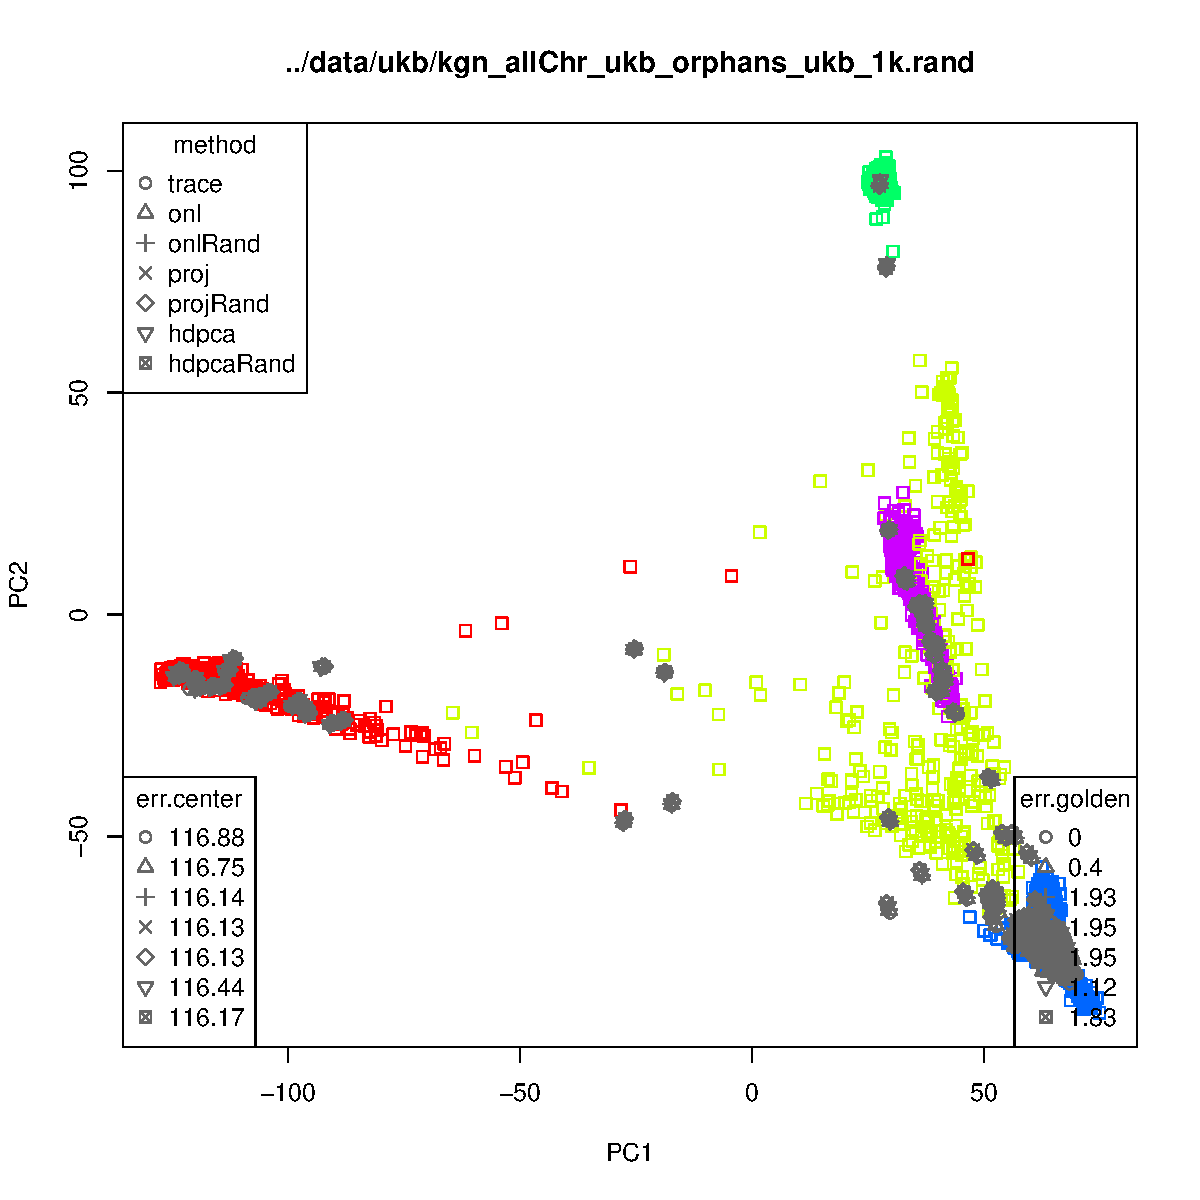
\includegraphics[width=0.98\textwidth]{ukb}
  \caption{
    The reference individuals are from the 1000 Genomes dataset with 2492 unrelated individuals from 5 superpopulations: African, American, East Asian, European, and South Asian. 
    The study sample contain 1000 individuals from the UKBioBank dataset.
    There are about 125,000 loci shared by the reference and study data.
    The golden standard error is the square root of the averate squared distance between the study individuals' PC scores predicted by different methods compared to the golden standard result, which in our case is the PC scores predicted by ADT.
  }
  \label{fig:ukb}
\end{figure}

\begin{figure}[p]
  \centering
  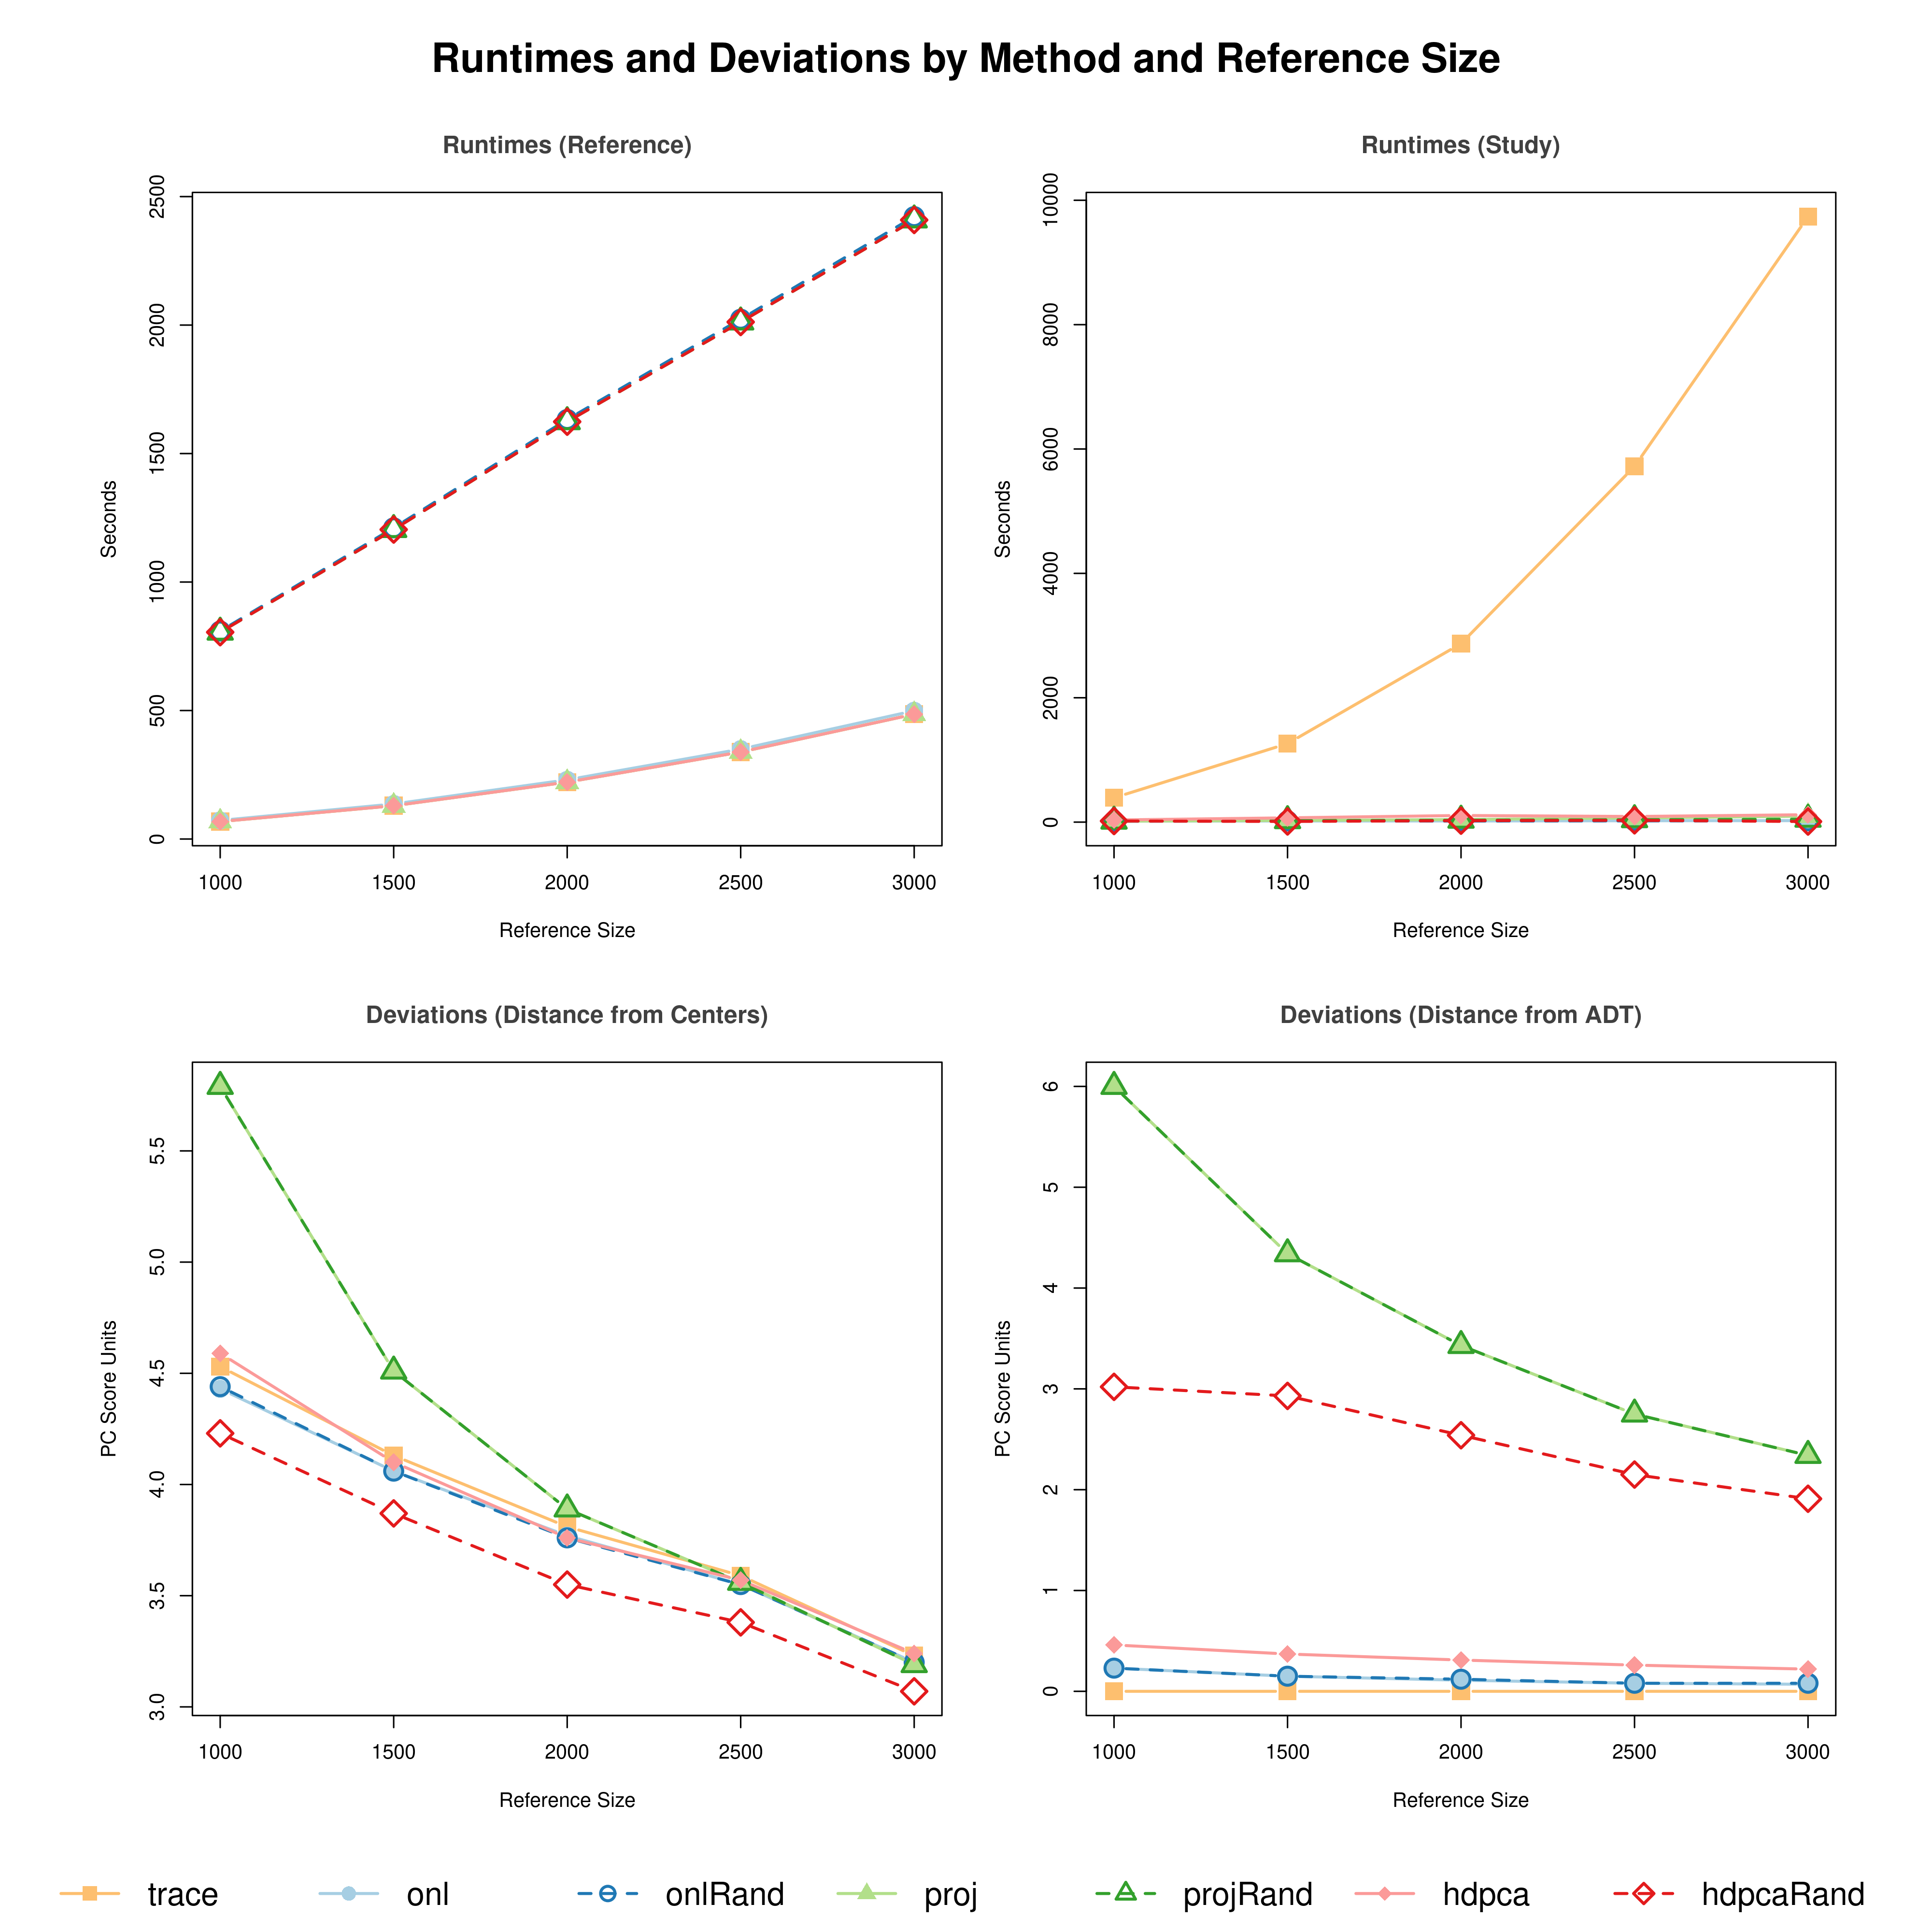
\includegraphics[width=0.98\textwidth]{nChg}
  \caption{
    Runtimes and deviations for different methods as the reference sample size increases.
    The study size is fixed to 200 and the number of SNPs is 100,000 (1000 per genealogy). 
    Simulation is done on a $2 \times 2$ grid with a migration rate of 100 by the GGS software. 
  }
  \label{fig:nChg}
\end{figure}

\begin{figure}[p]
  \centering
  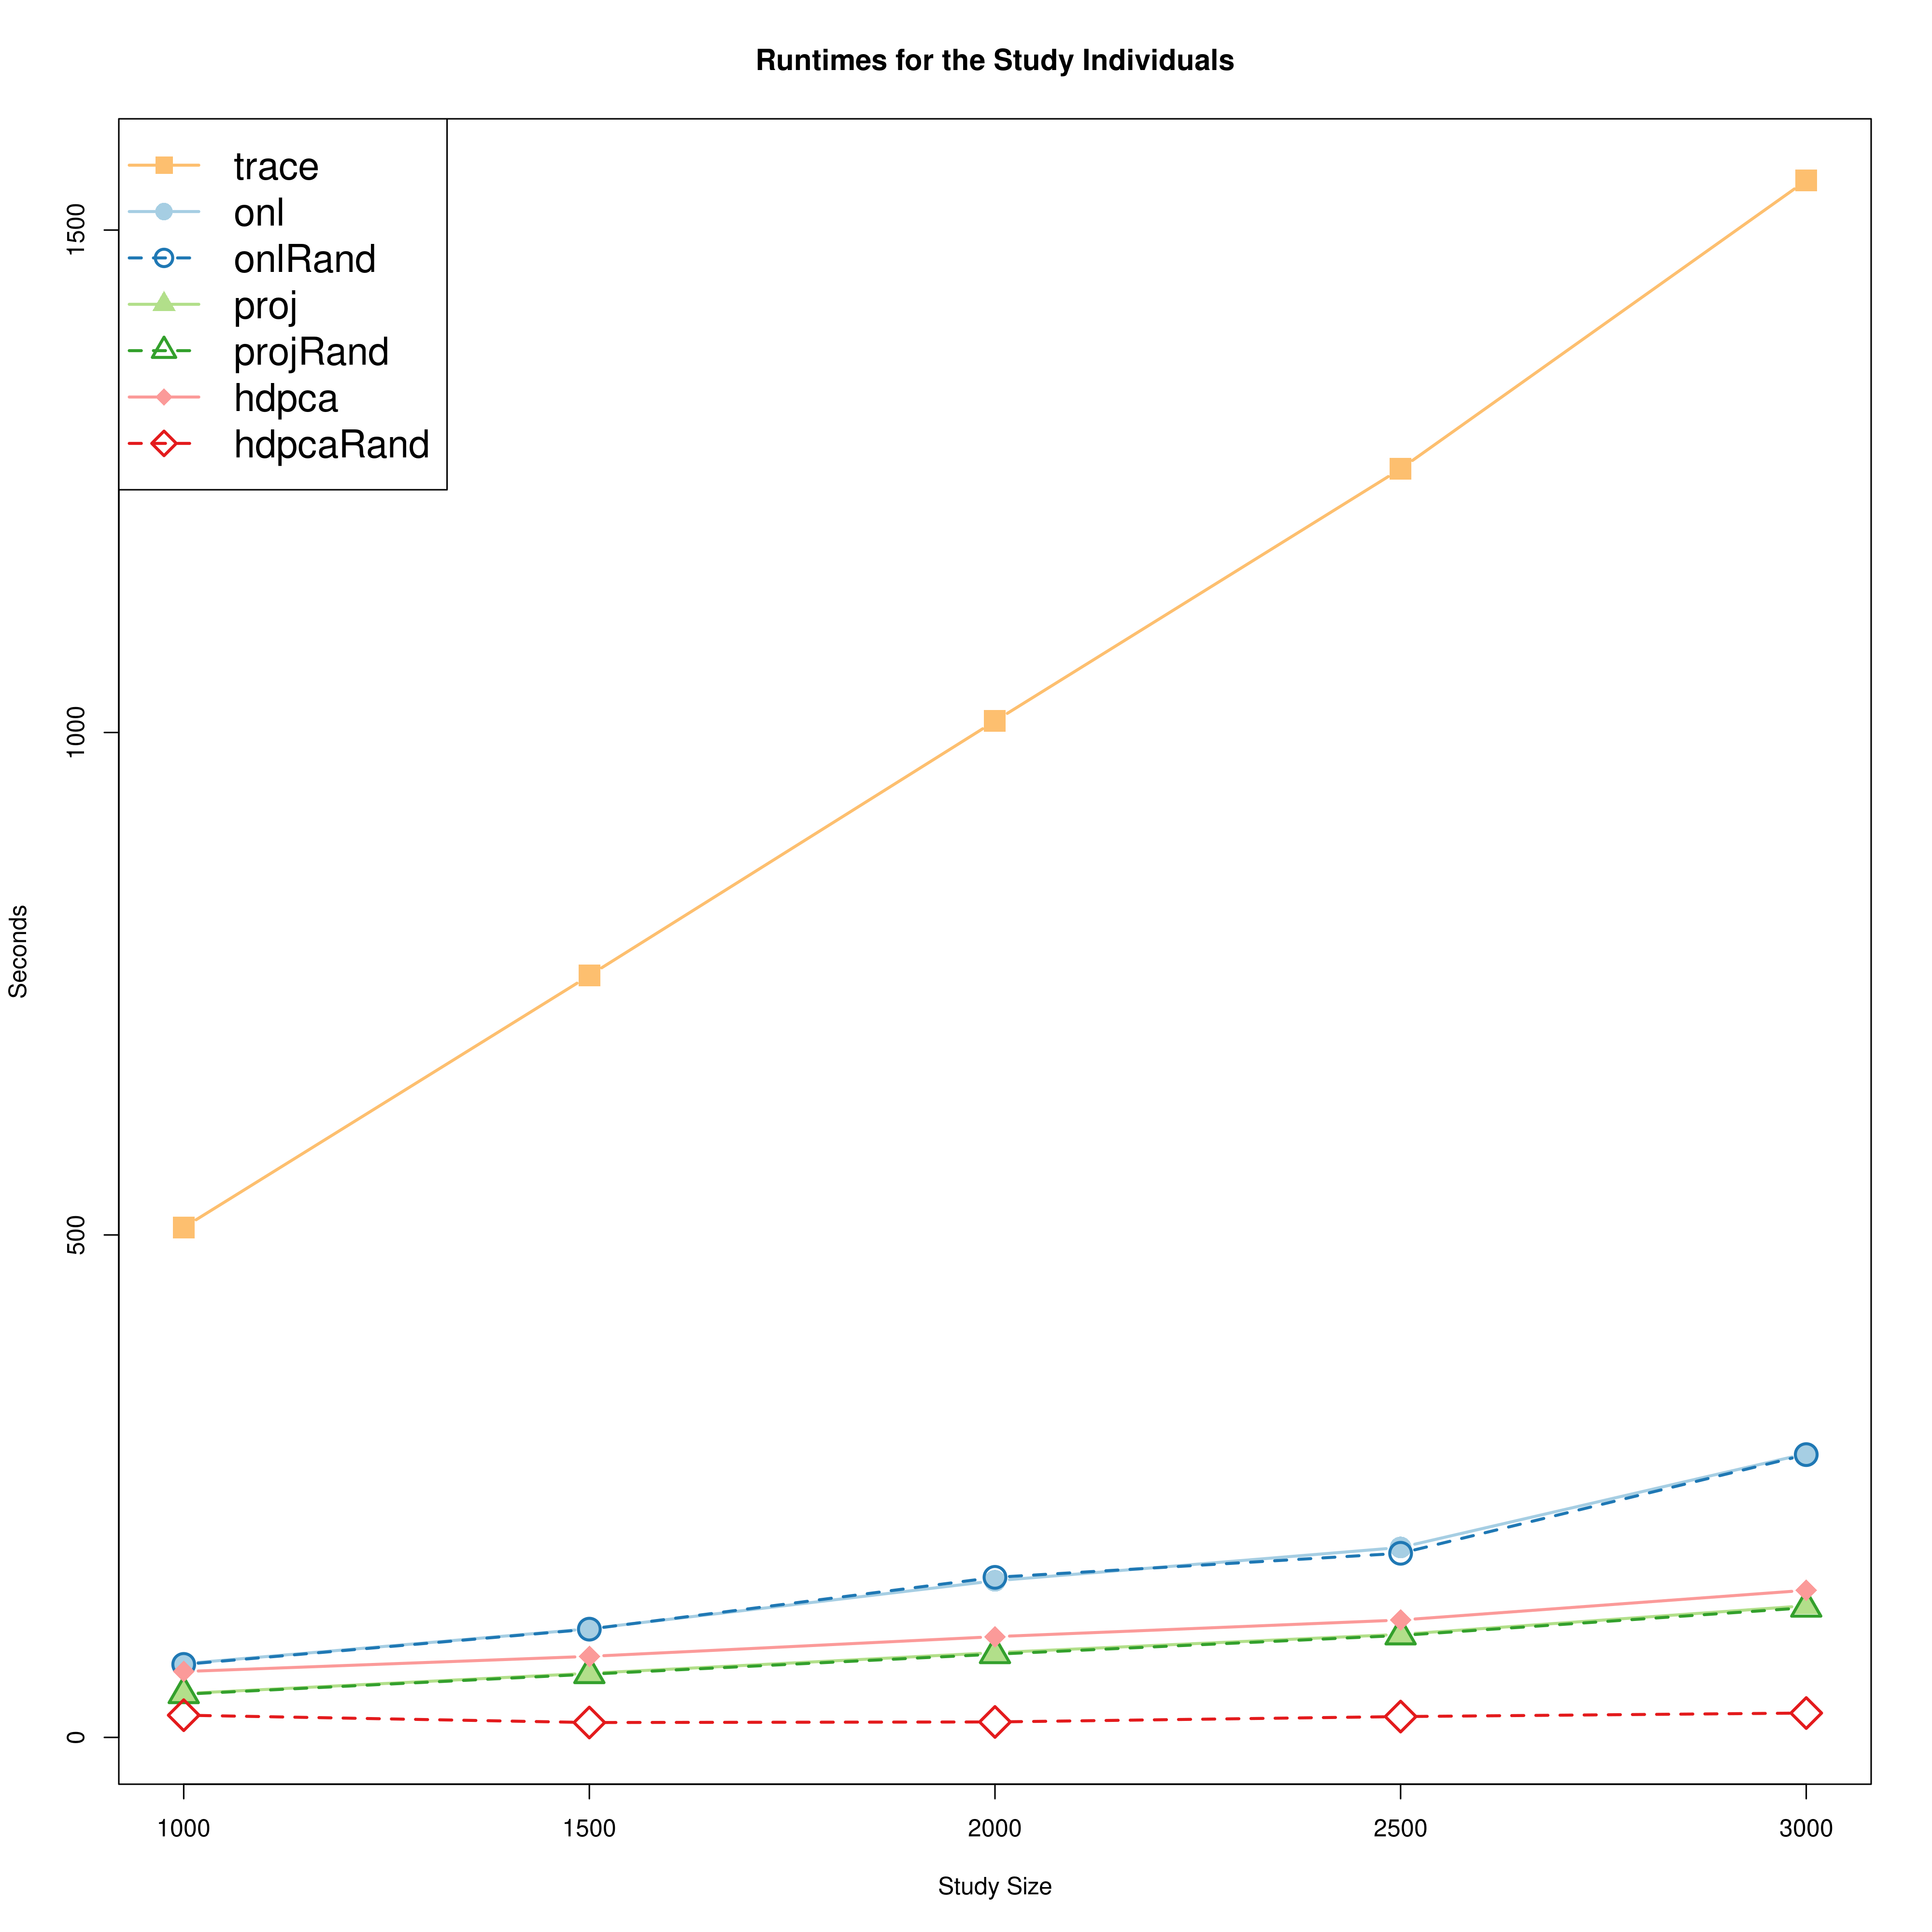
\includegraphics[width=0.98\textwidth]{mChg}
  \caption{
    Runtimes and deviations for different methods as the study sample size increases.
    The reference sample size is fixed to 600 and the number of SNPs is 100,000 (1000 per genealogy).
    Simulation is done on a $2 \times 2$ grid with a migration rate of 100 by the GGS software. 
  }
  \label{fig:mChg}
\end{figure}

% \includegraphics[width=0.98\textwidth]{runtimes_rand}

% \includegraphics[width=0.98\textwidth]{err_refcenter_rand}

% \includegraphics[width=0.98\textwidth]{err_trace_rand}

% \includegraphics[width=0.98\textwidth]{err_refcenter_rand}

% \includegraphics[width=0.98\textwidth]{kgn_allChr_ukb_orphans_ukb_1k_comb}

\newpage
 
% \includegraphics[width=0.98\textwidth]{kgn_allChr_ukb_orphans_ukb_1k_rand}

\newpage


\end{document}
